\section{INLA for Gaussian Data}
In this section we will look at the smoothing of a time series and how to use integrated nested Laplace approximations which we from here on will refer to as INLA.

\subsection{Data exploring}
 
\begin{figure}[h]
    \centering
    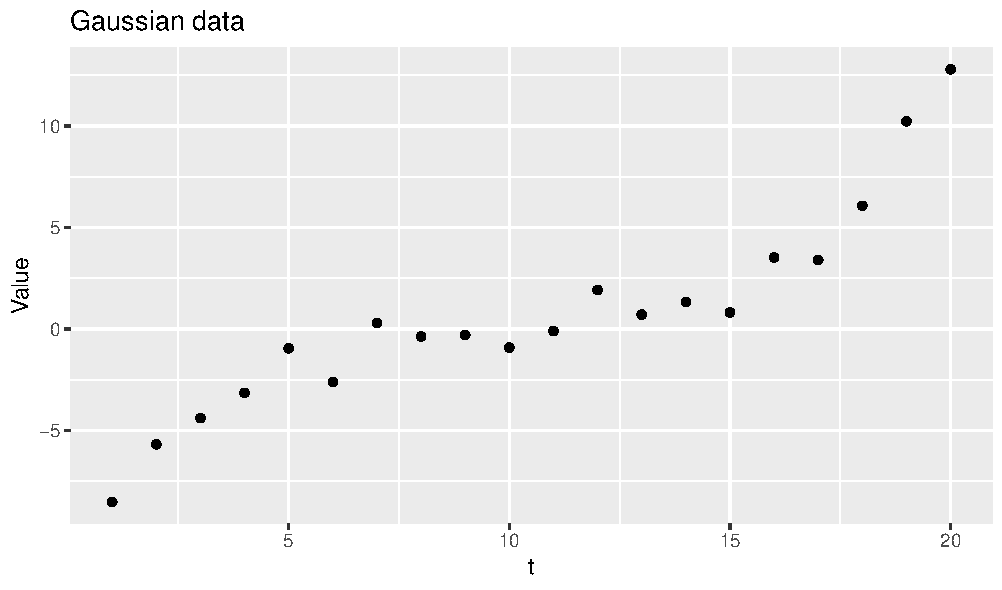
\includegraphics[width=\textwidth]{Images/gaussian_data.pdf}
    \caption{Constructed Gaussian data.}
    \label{fig:gaussian_data}
\end{figure}

In Figure \ref{fig:gaussian_data} vi can see the Gaussian data we want to find the underlying distribution of. We note that it looks like some of the previous values influence the next value in the time series. From the provided data, we have observations for $t = 1,...,20$, and this is what we will be using for the duration of this problem. 


\subsection{Latent Gaussian model}

As given in the problem text, we assume that given the vector $\eta = (\eta_1...\eta_{20})$ the observations $y_k$ are independent and Gaussian distributed, having mean $\eta_t$. The known unit variance is $y_t|\eta_t = \mathcal{N}(\eta_t, 1); t = 1,...,20$, and there is a smooth effect of time which the linear predictor is linked to, $\eta_t = f_t$. 

We are choosing a second order Random Walk model as the prior distribution for the vector \textbf{f} $= (f_1,...,f_{20})$ model the temporal effects of the covariates. As $\eta_t = f_t$, we have that 

\begin{align} \label{RW_prior}
    \pi(\mathbf{f}|\theta) = \pi(\mathbf{\eta}|\theta) \propto
    \theta^{(T-2/2)} \text{exp} \Bigg\{  -\frac{\theta}{2} \sum_{t = 3}^{20} (f_t - 2f_{t-1} + f_{t-2})^2  \Bigg\} = \mathcal{N}(\mathbf{0}, \mathbf{Q}(\theta)^{-1}).
\end{align}


To find the precision matrix for our model, we expand the expression for $\textbf{Q}(\theta)$ from equation \ref{RW_prior}. We then have that 

\begin{align} \label{precision_mat}
    \textbf{Q}(\theta) = \sum_{t = 3}^{20} (f_t - 2f_{t-1} + f_{t-2})^2 \nonumber \\
    = \sum_{t = 3}^{20} (f_t^2 + 4f_{t-1}^2 + f_{t-2}^2 - 4f_t f_{t-1} - 4 f_{t-1} f_{t-2} + 2f_t f_{t-2}) \nonumber \\
    = ... = 
    \begin{bmatrix}
        1 & -2 & 1 & . & . & . & . & . \\
        -2 & 5 & -4 & 1 & . & . & . & .  \\
        1 & -4 & 6 & -4 & 1 & . & . &  . \\
        . & 1 & -4 & 6 & -4 & 1 & . & . \\
        . & . & 1 & -4 & 6 & -4 & 1 & . \\
        . & . & . & 1 & -4 & 6 & -4 & 1 \\
        . & . & . & . & 1& -4& 5 & -2 \\
        . & . & . & . & . & 1 & -2 & 1 
    \end{bmatrix}.
\end{align}

This is a sparse matrix. As the precision matrix is sparse, and we assume the latent model to be Gaussian, this is a Gaussian Markov Random Field (GMRF). 


\todo[color = yellow]{Hvis du fokuserer på å få inn alle plottene og skrive innn likningene så kan jeg vet skrive forståelsestingene på tirsdag. I hvert fall er g6t5fr5det fint om du tar det i den rekkefølgen :D  }



A structured additive model can be defined as 

%Dette er structured additiv model
\begin{equation} 
\begin{split}
    g(\mu_i) = \eta_i = \alpha + \sum_{k = 1}^{n_\beta} \beta_k z_{mi} + \sum_{j = 1}^{n_f}f^{(j)}(u_{ji}) + \epsilon_i.
\end{split}
\end{equation}

As our model is a latent Gaussian model, and these are a subclass of the structured additive regression model, then $y$ belongs to the exponential family. In addition, all latent variables have Gaussian priors. In addition to this, the latent field has to be conditionally independent, and our model is conditionally independent given the $\eta$-vector. As all this is fulfilled in our model, along with the requirement that there are few hyperparameters, we can use INLA to estimate the model parameters. 




\subsection{Gibbs sampling algorithm for $f(\eta, \theta |y)$}
\label{Gibbs}

First we implement a Gibbs sampling algorithm for $f(\eta, \theta |y)$. To do so we need the full conditional of both $\pi(\theta|\eta, y)$ and $\pi(\eta|\theta, y)$. They are:

- skriv inn the full conditional for $\pi(\theta|\eta, y)$ og $\pi(\eta|\theta, y)$

\begin{align}
    \pi(\theta| \eta, y) = \pi(y|\eta) \cdot \pi(\eta|\theta) \cdot \pi(\theta) \propto \pi(\eta|\theta) \cdot \pi(\theta) \nonumber \\
    = \theta^{\frac{(T-2)}{2}} \cdot \text{exp} \Big\{ \eta^T Q \frac{\theta}{2} \eta \Big\} \cdot \text{exp}(\theta) \nonumber \\
    = \text{exp} \Big\{  \theta \big(1 + \frac{\eta^T Q \eta}{2}  \big) \theta^{\frac{(T-2)}{2}}  \Big\}, 
\end{align}

and 
\begin{align}
    \pi(\eta | \theta, y) \propto f(\mathbf{f}|\mathbf{\eta}) \cdot f(\mathbf{\eta}|\theta) \nonumber \\
    \propto \text{exp} \Bigg\{ -\frac{1}{2}(\mathbf{y} - \mathbf{\eta})^T I (\mathbf{y}-\mathbf{\eta}) - \frac{1}{2} \mathbf{\eta}^T Q \mathbf{\eta} \Bigg\} \nonumber \\
    = \text{exp} \Bigg\{  -\frac{1}{2} \Big[ (\eta - a)^T (I - Q) (\eta - a) \Big] \Bigg\}, 
\end{align}

with $a = y(I + Q \theta)^{-1}$ and $\sum = (I + Q \theta)^{-1}$. 

We note that the full conditional for $\theta$ is a gamma distributed with shape parameter $\alpha = T/2$ and scale parameter $\beta = 1/(\frac{1}{2}\cdot (1 + \eta^T Q \eta))$ and the full conditional for $\eta$ is multivariate normal distributed with mean $\boldsymbol{\mu} = \boldsymbol{y}(I + Q \theta)^{-1}$ and variance covariance matrix given by $\Sigma = (I + Q \theta)^{-1}$. $Q$ is the precision matrix defined in  \ref{precision_mat}....
$I$ is the identity matrix and $y$ are the values of the dataset for each time as seen in Figure \ref{fig:gaussian_data}. 


\lstinputlisting[language=R, firstline=56, lastline=67]{Code/INLA.R}

Now we are ready to implement the Gibbs sampling for $f(\eta, \theta | \boldsymbol{y})$. Firstly, we propose a new value for $\theta$ using the full conditional $\pi(\theta|\eta, \boldsymbol{y})$ then we propose a new value for $\eta$ using the full conditional $\pi(\eta|\theta, \boldsymbol{y})$. 

\lstinputlisting[language=R, firstline=69, lastline=86]{Code/INLA.R}

We run with initial values for $\theta = 0$ and $\eta$ a random sample from the ful lconditional of $\eta$ given the initial condition for $\theta$.

\lstinputlisting[language=R, firstline=88, lastline=100]{Code/INLA.R}

Since this is an MCMC algorithm we need to evaluate the burn in period. 

\begin{figure}
    \centering
    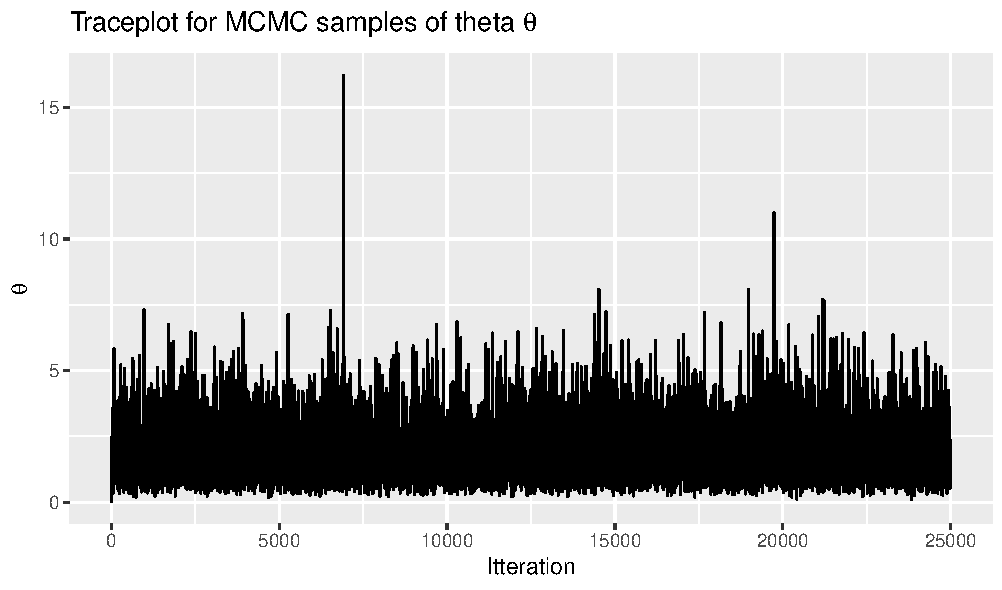
\includegraphics[width = \textwidth]{Images/trace_theta_mcmc.pdf}
    \caption{Traceplot for $\theta$ using Gibbs sampling}
    \label{fig:trace_theta}
\end{figure}

We can see from Figure \ref{fig:trace_theta} that the algorithm seems to converge very fast. It has one spike around $iteration= 7000$ so we decide to discard the first $10 000$ samples. When we explore the trace plot for all $\eta_i$ non of them has a longer burn in period and all seem to converge very fast. This is also as expected since the Gibbs sample draws from the actual full conditional. 

%%%%%%%%%%%%%%%%%%%%%%%%%%%%%%%%%%%%%%%%%%%%%%%%%%%%%%%%%%%%%%%%%%%%%%%%%%%%%%%%%%%%%%%%%%%
%%%%%%%%%%%%%%%%%%%%%%%%%%%%%%%%%%%%%%%%%%%%%%%%%%%%%%%%%%%%%%%%%%%%%%%%%%%%%%%%%%%%%%%%%%%
\subsubsection{Estimate for the posterior marginal for the hyperparameter $\pi(\theta|y)$}

\begin{figure}[h!]
    \centering
    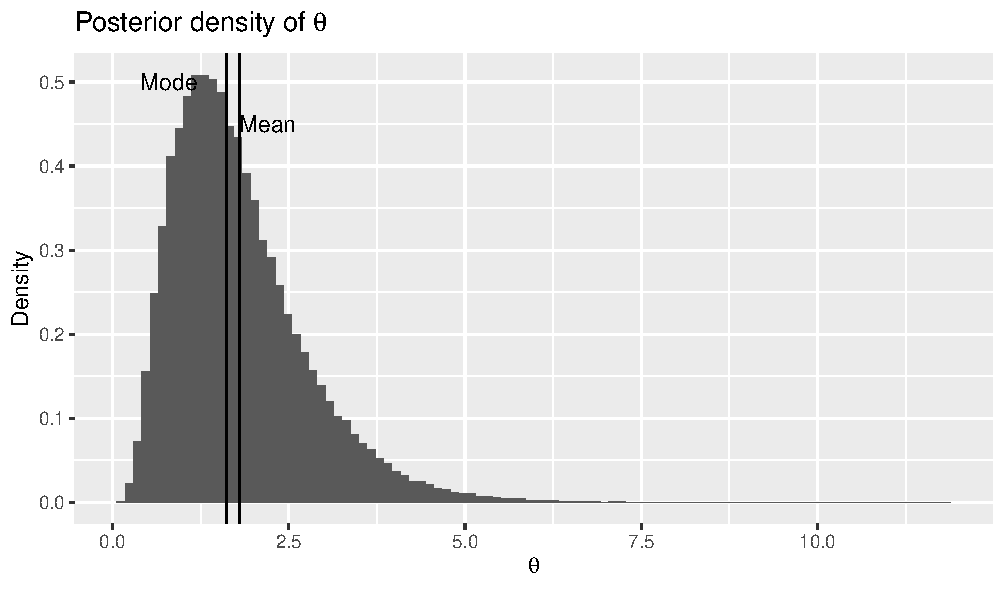
\includegraphics[width=\textwidth]{Images/post_theta_mcmc.pdf}
    \caption{Plot of the estimate for the posterior marginal for the hyperparameter $\pi(\theta|y)$.}
    \label{fig:post_theta_mcmc}
\end{figure}

After discarding the burn in period we get the posterior distribution for $\pi(\theta|y)$. This can be seen in Figure \ref{fig:post_theta_mcmc}. 

%%%%%%%%%%%%%%%%%%%%%%%%%%%%%%%%%%%%%%%%%%%%%%%%%%%%%%%%%%%%%%%%%%%%%%%%%%%%%%%%%%%%%%%%%%%
%%%%%%%%%%%%%%%%%%%%%%%%%%%%%%%%%%%%%%%%%%%%%%%%%%%%%%%%%%%%%%%%%%%%%%%%%%%%%%%%%%%%%%%%%%%
\subsubsection{Estimate of the smooth effect using the mean and pointwise a $95 \%$ confidence bound around the mean}

\begin{figure}[h]
    \centering
    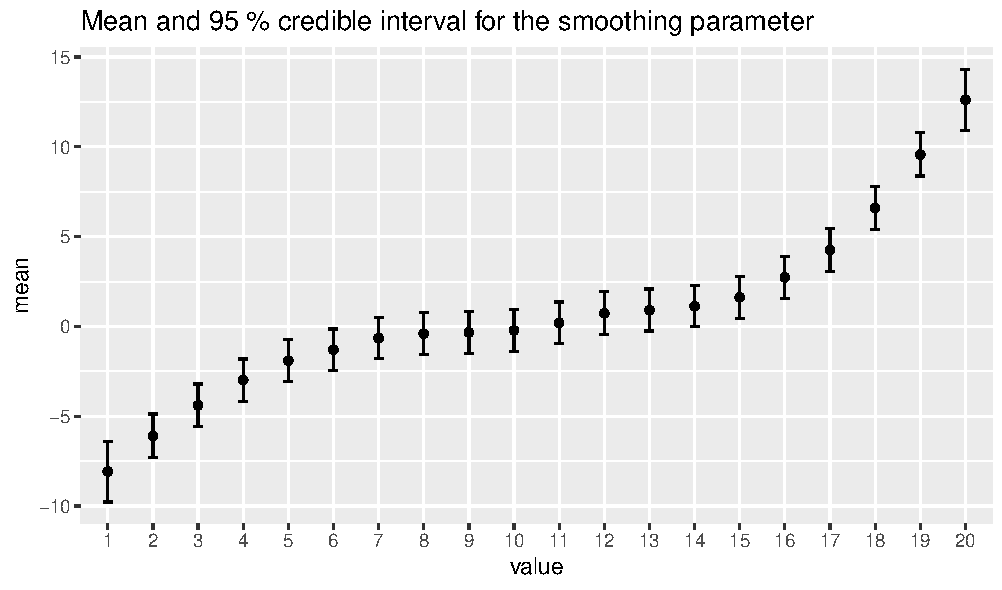
\includegraphics[width=\textwidth]{Images/post_eta_mcmc.pdf}
    \caption{Plot of the mean and the $95\%$ credible interval for the smoothing parameter $\eta$. }
    \label{fig:post_eta_mcmc}
\end{figure}

We can also look at the mean and $95 \%$ credible intervals. This can be seen in Figure \ref{fig:post_eta_mcmc}.


%%%%%%%%%%%%%%%%%%%%%%%%%%%%%%%%%%%%%%%%%%%%%%%%%%%%%%%%%%%%%%%%%%%%%%%%%%%%%%%%%%%%%%%%%%%
%%%%%%%%%%%%%%%%%%%%%%%%%%%%%%%%%%%%%%%%%%%%%%%%%%%%%%%%%%%%%%%%%%%%%%%%%%%%%%%%%%%%%%%%%%%
\subsection{Approximating the posterior marginal for the hyperparameter $\theta$, $\pi(\theta|y)$ using the INLA scheme}
\label{theta_post_inla}

We now want to use the INLA scheme to find the posterior for $\pi\theta| \boldsymbol{y})$ and $\pi(\eta_i| \boldsymbol{y})$ for all $i$.

- Sett inn likningn fra opgaven

To find the posterior for $\theta$, we begin with

\begin{align}\label{post_theta}
    \pi(\theta|\mathbf{y}) \propto \frac{\pi(\mathbf{y}|\eta,\theta)\pi(\eta|\theta)\pi(\theta)}{\pi(\eta|\theta, \mathbf{y})}.
\end{align}

We see from equation \ref{post_theta} that we need $\pi(\boldsymbol{y}| \eta, \theta)$. We have that 

\begin{align}
    \pi(\mathbf{y}| \eta, \theta) = \pi(\mathbf{y}|\eta),  
\end{align}


which is multivariate normal distributed. 

We also need to find $\pi(\theta, \eta)$. This is given by 

\begin{align}
  \pi(\theta, \eta) = \pi(\eta|\theta)\pi(\theta)
  = 
\end{align}




We note this is a gamma distribution with rate parameter $\alpha = 1$ and scale parameter $\beta = \frac{1}{1 + \frac{1}{2} \eta^{T} Q \eta}$

Lastly we need $\pi(\eta| \theta \boldsymbol{y})$ which we calculated in part \ref{Gibbs} to be a gamma distribution with rate, $\alpha = \frac{T}{2}$ ans scale parameter $\beta = 1/(\frac{1}{2}\cdot (1 + \eta^T Q \eta))$ 

We constuct a grid for values of $\theta$ chose an $\eta$ at random since this should be true for all $\eta$ and compute all the elements mentioned above.  

\lstinputlisting[language=R, firstline=177, lastline=186]{Code/INLA.R}

\lstinputlisting[language=R, firstline=188, lastline=197]{Code/INLA.R}

We now have the approximation for the porsterior density of $\theta$.
\begin{figure}[h!]
    \centering
    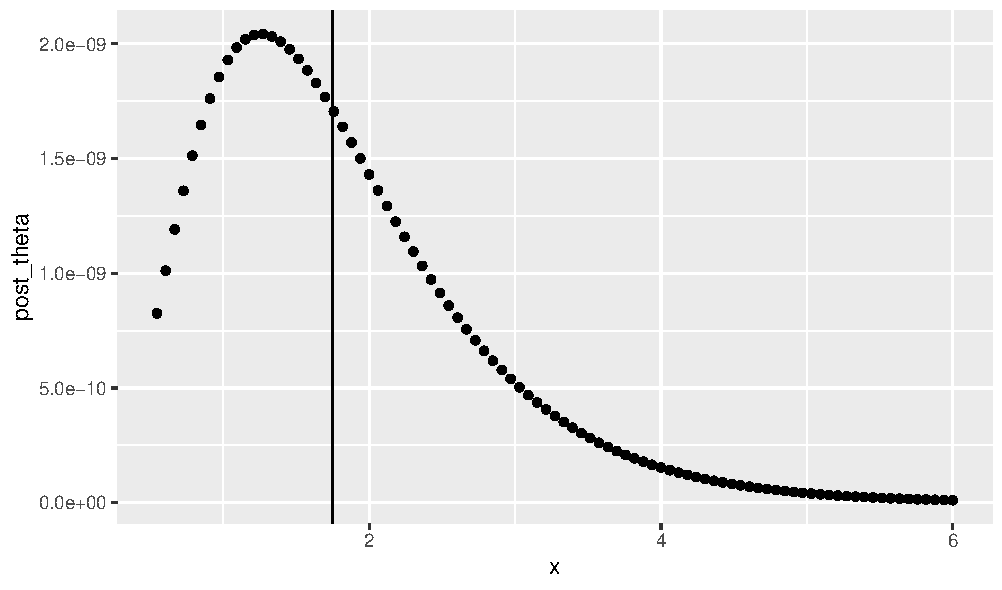
\includegraphics[width=\textwidth]{Images/post_theta_inla.pdf}
    \caption{Plot of the estimate for the posterior marginal for the hyperparameter $\pi(\theta|y)$ using the INLA scheme.}
    \label{fig:post_theta_inla}
\end{figure}

Figure \ref{fig:post_theta_inla} shows the posterior distribution computed by INLA. We note that this should be multiplied by a normalizing constant. However this will only shift the values of the density not the shape. 
%%%%%%%%%%%%%%%%%%%%%%%%%%%%%%%%%%%%%%%%%%%%%%%%%%%%%%%%%%%%%%%%%%%%%%%%%%%%%%%%%%%%%%%%%%%
%%%%%%%%%%%%%%%%%%%%%%%%%%%%%%%%%%%%%%%%%%%%%%%%%%%%%%%%%%%%%%%%%%%%%%%%%%%%%%%%%%%%%%%%%%%

\subsubsection{Implementing the approximation of the marginal posterior for the smooth effect, $\pi(\eta_i | y)$}

We now want to preform tha last inla step, implementing the approximation of the marginal posterior for the smooth effect, $\pi(\eta_i | y)$ We will do this only for $\eta_{10}$. 

We know 

\begin{equation}
\label{eq:eta_post}
    \pi(\eta|\boldsymbol{y}) = \int \pi(\eta|\boldsymbol{y}, \theta) \pi(\theta|\boldsymbol{y}) d\theta.
\end{equation}

In order to approximate \eqref{eq:eta_post} we compute $\pi(\eta|\boldsymbol{y}, \theta) \pi(\theta|\boldsymbol{y})$ for a grid of eta values for all values in the $\theta$-grid from Section \ref{theta_post_inla}. We use the values for $\pi(\theta|\boldsymbol{y})$ computed earlier. Finaly we sum all the weighted densities for $\pi(\eta|\boldsymbol{y}, \theta)$ weighted by $\pi(\theta|\boldsymbol{y})$

\lstinputlisting[language=R, firstline=221, lastline=227]{Code/INLA.R}

\lstinputlisting[language=R, firstline=232, lastline=240]{Code/INLA.R}

\lstinputlisting[language=R, firstline=244, lastline=244]{Code/INLA.R}

\begin{figure}
    \centering
    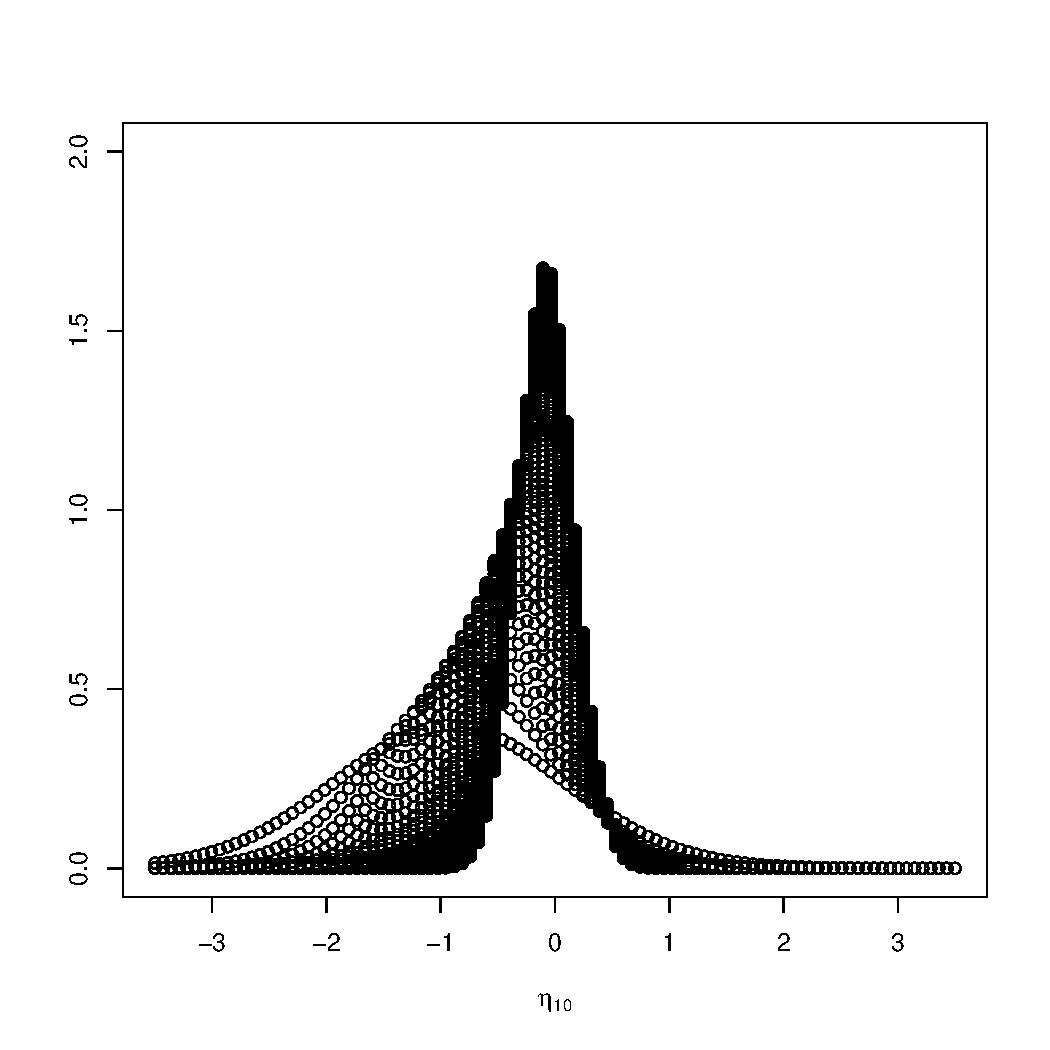
\includegraphics[width=\textwidth]{Images/eta_10.pdf}
    \caption{All distributions of $\eta_{10}$ given $\theta$ from the grid as given in Section \ref{theta_post_inla}}
    \label{fig:eta_all}
\end{figure}


In Figure \ref{fig:eta_all} we can see all $\pi(\eta_{10}|\theta, \boldsymbol{y})$. To get  $\pi(\eta_{10}|\theta)$ we sum them all weighted by $\pi(\theta|\boldsymbol{y})$. 

\begin{figure}[h!]
    \centering
    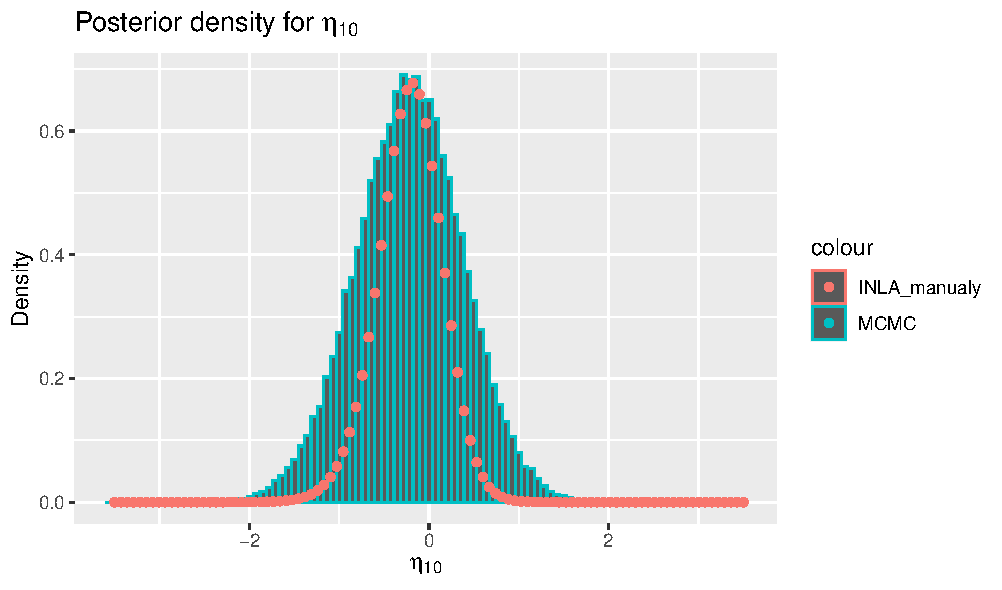
\includegraphics[width=\textwidth]{Images/post_eta_inla.pdf}
    \caption{Plot of the estimate for the posterior marginal for the smoothing effect $\pi(\eta_i|y)$ using the INLA scheme.}
    \label{fig:post_eta_inla}
\end{figure}

This gives us the density seen in Figure \ref{fig:post_eta_inla} together with the posterior computed by the Gibbs sampler earlier. As we can see these do not completely overlap. The one using INLA is slightly slimmer. We did not have the time to further research why this error occurred.

%%%%%%%%%%%%%%%%%%%%%%%%%%%%%%%%%%%%%%%%%%%%%%%%%%%%%%%%%%%%%%%%%%%%%%%%%%%%%%%%%%%%%%%%%%%
%%%%%%%%%%%%%%%%%%%%%%%%%%%%%%%%%%%%%%%%%%%%%%%%%%%%%%%%%%%%%%%%%%%%%%%%%%%%%%%%%%%%%%%%%%%
\subsection{Using the inla() - function in R to implement the model,and comparing the results}

Finally we use the inla function from the R package R inla to implement the same model. 

\lstinputlisting[language=R, firstline=269, lastline=280]{Code/INLA.R}

We compare this with our previous distributions.
\begin{figure}[h]
    \centering
    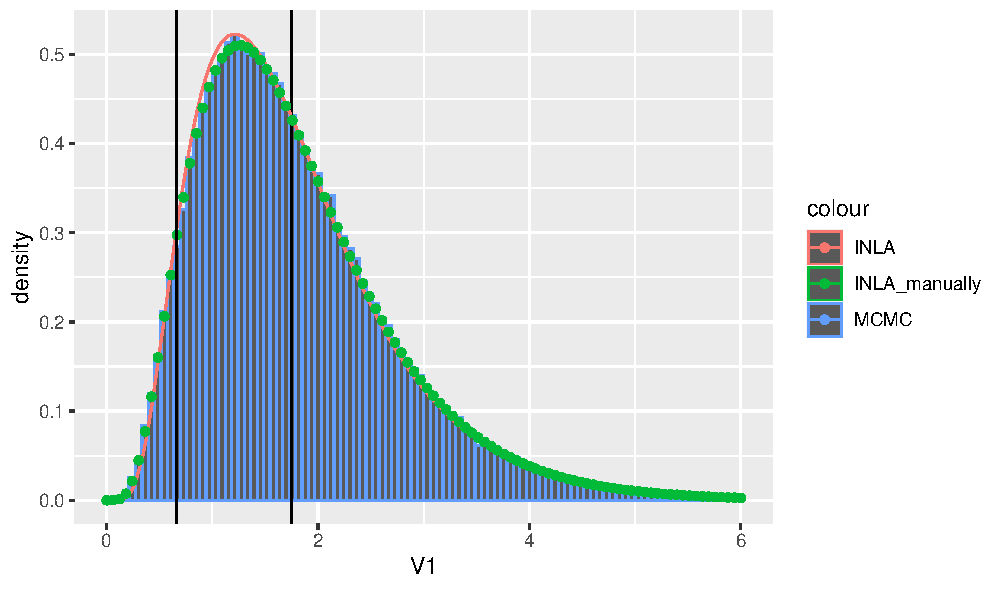
\includegraphics{Images/theta_comparison.pdf}
    \caption{Plot of estimated hyperparameter $\theta$ for MCMC, manually implemented INLA and INLA implemented using R-inla().}
    \label{fig:theta_comparison}
\end{figure}

From Figure \ref{fig:theta_comparison} we see that the distribution overlaps perfectly. We note here that we scaled the manualy computed INLA posterior by $0.9*10^7$ and consider this the normalizing constant. We should probably have computed this more propparly but since we had limited amount of time we chose not to focus on this. 

\begin{figure}[h]
    \centering
    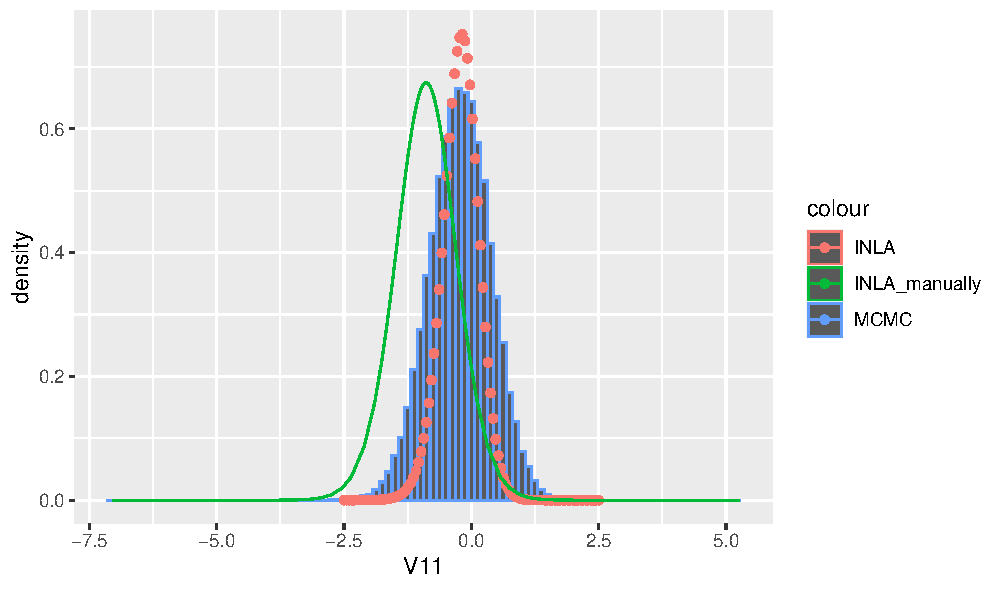
\includegraphics{Images/smoothing_comparison.pdf}
    \caption{Plot of estimated smoothing parameter $\eta$ for MCMC, manually implemented INLA and INLA implemented using R-inla().}
    \label{fig:smoothing_comparison}
\end{figure}

In Figure \ref{fig:smoothing_comparison} we see all three posterior distributions for $\eta_{10}$ and see that they do not overlap as expected. We see that the posterior computed by R.INLA looks slimilar to the one from the gibs sampling but shifted slightly to the left. 

In fact when we shift this distribution to the right by $0.65$ they overlap perfectly. 

We therefor make a plot to compare the distribution for all $\eta_i$ from both hte Gibbs sampler and the R-inla posteriors. This is shown in figure ..... We see that it looks like the Gibbs sampler is consequently lower than R inla. We note however that the lenght of the credible intervals look very similar and the shift is consistent over all $eta_i$. Hence we think the error might ly in the mean of the computation of $eta_i$ in the Gibbs sampler.  